\documentclass[letterpaper, 10 pt, conference]{ieeeconf}  % Comment this line out
\IEEEoverridecommandlockouts                              % This command is only
% needed if you want to
% use the \thanks command
\overrideIEEEmargins
\usepackage[ruled,lined,linesnumbered]{algorithm2e}
\newtheorem{remark}{Remark}[section]


\newcommand{\bs}{\boldsymbol}
\usepackage{graphicx}
\usepackage[font=small,labelfont=bf]{caption}
\usepackage{subcaption}

% \IEEEoverridecommandlockouts                              % This command is only
% \overrideIEEEmargins
\usepackage{amssymb,amsmath}
% \usepackage{mathtools}
\usepackage{hyperref}
\newtheorem{Lemma}{Lemma}

% correct bad hyphenation here
\hyphenation{op-tical net-works semi-conduc-tor}

\begin{document}
\title{\LARGE \bf
Reactive control of a dual-arm ping-pong ball juggling robot
}
\author{
  Yuquan Wang 
  \thanks{
    e-mail: \tt{ $\{$yuquan$\}$@kth.se}}
}

\maketitle
\thispagestyle{empty}
\pagestyle{empty}

\begin{abstract}
This report summarizes a pingpong-ball juggling control strategy for a dual-arm robot. We assume that each arm has 7 Degrees of freedom (DOF) and the robot end-effector is a racket. 

Assuming that the perception (vision) system is able to provide accurate estimate of the ball trajectories, we use constraint-based programming to reactively control the robot such that the robot is able to handle the in-herent randomness of such a pingpong-ball paddling task. 


In the preliminery experimental validation, we model the striking process with simplifed flight dynamics and impact dynamics. 

\end{abstract}

% \begin{keywords}
%   parallel and branching structure; virtual kinematic chain; constraint-based programming;
% \end{keywords}
\IEEEpeerreviewmaketitle

% ===============================================================================
\section{Introduction }
\label{sec:intro}
Cascade juggling of more than one ball combines deterministic process with random fluctuations \cite{post2000principal}. The control or stabilization of such an inherent stochastic system requires sensory feedback in real time. 

% We can also find from \cite{post2000principal} that 

Constraint based programming provides a versatile framework for combining several different constraints into a single robot control scheme \cite{de2007constraint}.
We take advantage of the redundancy of  a robot manipulator to improve the execution of a reactive tracking task. Particularly due to the dexerity demand from  more than one pingpong ball, we explore the redundancy of the robot by formulating proper task-dependent measures and/or constraints and integrating them with an optimization framework \cite{wangIFAC2014}. 


% why not catch and throw... 


The rest of the report is organized as follows: we introduce how we model the juggling with certain assumptions in Sec.~\ref{sec:modelling}, we propose an reactive control strategy in  Sec.~\ref{sec:control} and we conclude this report by introducing the experimental setup in Sec.~\ref{sec:experiment}




% While the increasing randamness could reduce the controllability of a system, it may also be useful to avoid staying at locally optimal solutions.


   



\section{Modelling}
\label{sec:modelling}

\subsection{Flight and impact dynamics }
\label{sec:dynamics}
We are not aiming for using a robot hand which is able to open or close  fingers \cite{kober2012playing}, instead we simplify the catch/throw as paddling.   
According to the early pioneers in \cite{rizzi1992distributed}, 
we should model the
striking process with proper flight dynamics of the ball and the impact dynamics
between the ball and the racket. 

Baically we can model the ball as point mass under gravity force using the following state space model: 
\begin{equation}
\label{eq:ss_ball_dynamics}
\begin{bmatrix}
  \dot{\bs{b}}\\ 
  \ddot{\bs{b}}
\end{bmatrix}
=
 \begin{bmatrix}
       0 & I           \\[0.3em]
       0 & 0
     \end{bmatrix}
\begin{bmatrix}
  \bs{b}\\ 
  \dot{\bs{b}} 
\end{bmatrix}
+
\begin{bmatrix}
  0\\ 
  \bs{g}
\end{bmatrix}
\end{equation}
where $\bs{b}\in\mathbb{R}^3$ represents the position of the ball and $\bs{g} = [ 0, 0, -9.8]^\top$ denotes the gravity force. 
We can construct an oberver of the flighting ball dynamics by feeding the discrete version of \eqref{eq:ss_ball_dynamics} as a state space model into a Kalman filter.  

We assume that components of the ball's velocity tangent to the plane of impact remains unchanged after the impact. Along the normal direction of the impact plane, we define a positive restitution coefficient $\alpha$ to model the impact dynamics: 
\begin{equation}
\label{eq:impact}
(\dot{\bs{b}}'_n - \bs{v}'_n )= -\alpha(\dot{\bs{b}}_n - \bs{v}_n),
\end{equation}
where $\bs{b}'_n$ and $\bs{v}'_n$ denote the normal components of the ball and paddle velocites right after impact, while  $\dot{\bs{b}}_n$ and $\bs{v}_n$ are prior to impact \cite{rizzi1992distributed}. 

Taking the robot inertia into account, we can assume that paddle is way heavier than the ball such that $\bs{v}'_n = \bs{v}_n$. Then we can simplify \eqref{eq:impact} as: 
\begin{equation}
\label{eq:impact_new}
\dot{\bs{b}}'_n = \dot{\bs{b}}_n + (1 + \alpha) (\bs{v}_n - \dot{\bs{b}}_n).
\end{equation}
\subsection{Dual-arm motion and the Juggling strategy}
\label{sec:dual-arm}
From the principal components in three-ball cascade juggling 
\cite{post2000principal},
we know that the candidate trajectory of the two end-effectors of a dual-arm robot resembles the trajectory shown in  Fig.~\ref{fig:trajectory}.
\begin{figure}[htbp]
  \begin{center}
    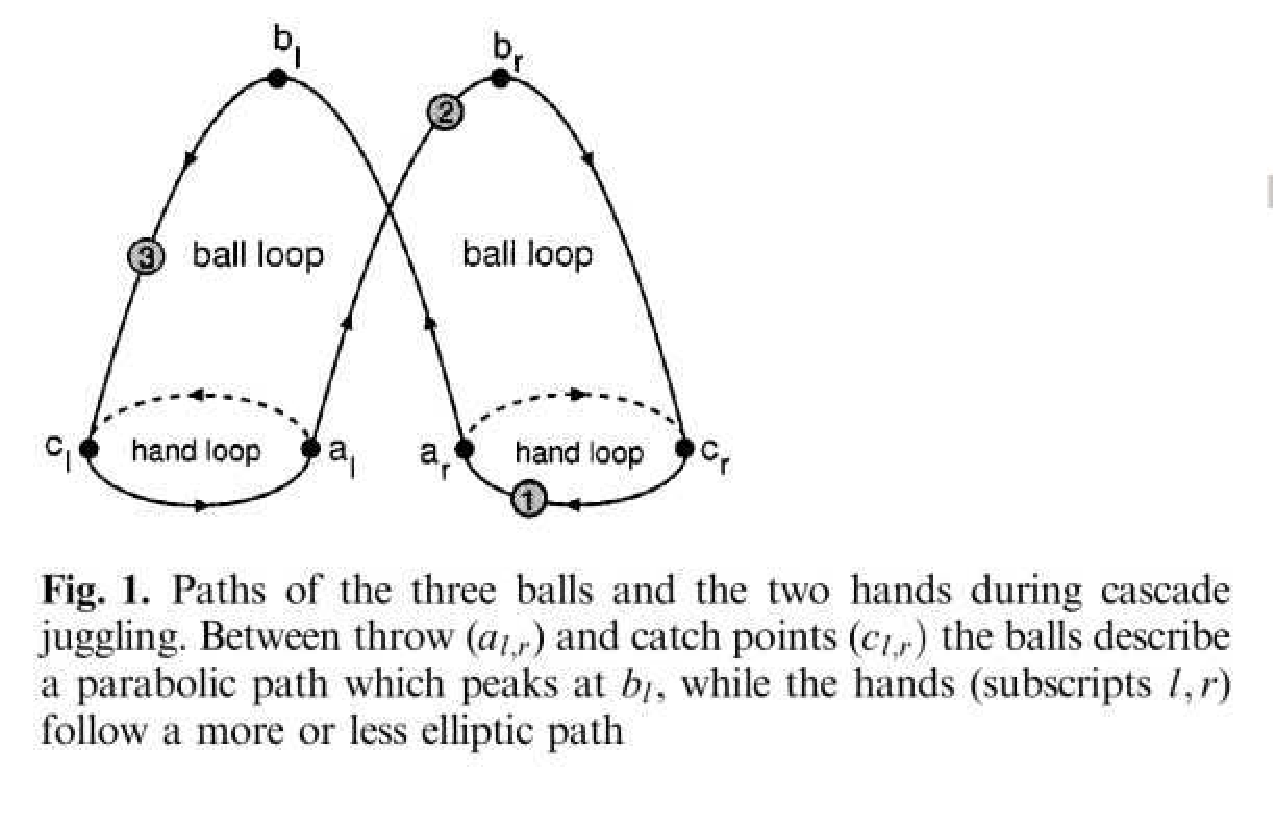
\includegraphics[width=1.0\columnwidth, height=0.7\columnwidth]{fig/trajectory}
    \caption{
      Fig.1 taken shamelessly from \cite{post2000principal}
    }
     \label{fig:trajectory}
  \end{center}
\end{figure}

We can summarize from Fig.~\ref{fig:trajectory} that 
the coordination of the two arms primarily depends on the throwing/catching. As the common robot arm consists of several revolute joints, we can use cyclic motion to model the end-effector(hand) loop. 

Using the aforementioned flight dynamics we can construct an observer of the ball trajectories with a Kalman filter, based on which we can online regulate the coordination of the two arms. 


As we earlier assumed in Sec.~\ref{sec:dynamics} that the catch/throw is simplifed as paddling, we can use a similar strategy as shown in Fig.~\ref{fig:new_trajectory}  
\begin{figure}[htbp]
  \begin{center}
    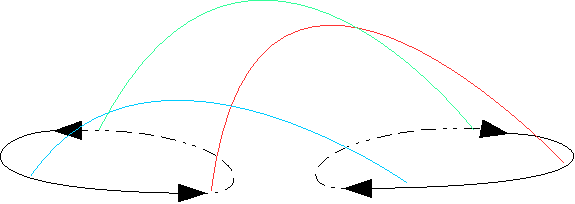
\includegraphics[width=1.0\columnwidth]{fig/trajectory_new}
    \caption{By simplifing the cathc/throw with elastic collision between ball and racket, we can assign three collisions on the trajectory of each of  the end-effectors. The tree distinct trajectories are marked with red-green-blue colors.
    }
     \label{fig:new_trajectory}
  \end{center}
\end{figure}

\section{Reactive control solution}
\label{sec:control}
We decompose the control problem for each arm in different aspects in Sec.~\ref{sec:specification} and based on which we explain how to formate an optimization problem in Sec.~\ref{sec:integration}.
\subsection{Constraints specification}
\label{sec:specification}
As we do not restrict the moving space of the ball, we can not apply the  mirror algorithm \cite{buehler1994planning} to paddle the ball. 
As shown in Fig.~\ref{fig:new_trajectory}, within one cycle of the $i$th paddle the $j$th ball has a nominal position $\bs{b}^{i}_j$ to impact with the $i$th paddle.  
Each nominal position is associated with a nominal direction $\bs{n}^i_j$. 

Using the  Kalman filter based on \eqref{eq:ss_ball_dynamics}, we can predict the state of the ball and therefore we can calculate the position error $\bs{e_{\bs{b}}}$  and the orientation error $\bs{e_{\bs{n}}}$. The position error $\bs{e_{\bs{b}}}$ could be calculated by directly taking the difference $\hat{\bs{b}}^{i}_j - \bs{b}^{i}_j$. We can use the direct design $\dot{\bs{e}} = -k \bs{e}$  to move the center of the racket to the landing position of the ball. 

The orientation error
 $\bs{e_{\bs{n}}}$ could be defined by unit quaternions, see \cite{yuquan2015}. Basically the idea is to use $\bs{e_{\bs{n}}}$ to adjust the racket orientation such that the parabola of the ball points to the prespecified position.

Using the prespecified impact model and unit quaternion, we intuitively realize the correction with the following: 
\begin{equation}
{\bs{n}^{i}_j}'  =
 \frac{-\hat{\bs{n}}^{i}_j + \bs{n}_r  }{2},
\end{equation}
where ${\bs{n}^{i}_j}'$ denotes the diretion of the ball after impact,
$\hat{\bs{n}}^{i}_j $ denotes the direction of the ball prior to the impact, $\bs{n}_r$ denotes the normal direction of the racket. 

As pointed out by \cite{post2000principal} and constaint-based programming papers, e.g. \cite{mansard2009unified}, the smooth transition between constraints is important yet not easy to obtain. We can use change the translation and orientation by following timed sinus wave to achive a smoother transition. 

% As there are multiple balls, we 

% We prioritize the three juggling tasks using the cloest distance between the ball and the racket. 

\subsection{Constraints integration}
\label{sec:integration}
Suppose there are 
task-dependnet constraints and objectives  $\eta_0$, $\boldsymbol{\eta}_1$ and $\eta_2$, we can calculate the motion of the robot end-effectors by formulating and solving optimization problems as:
\cite{wangIFAC2014} 
\begin{equation*}
\begin{aligned}
% \label{eq:qp_formulation}  
\min_{\dot{\bs{\theta}}, \nu^2_{i=0,1,2}} & \frac{\partial \eta_3}{\partial \boldsymbol{\theta}}^{\top}\dot{\boldsymbol{ \theta}}+\dot{\boldsymbol{ \theta}}^{\top}Q\dot{\boldsymbol{ \theta}}
% +\sum_{i=0,2}w_i\nu^2_i
% =======
% \begin{eqnarray*}
%   \min_{\dot{\bs{\theta}}, \nu^2_{i=0,1,2}} && -\frac{\partial \eta_3}{\partial \boldsymbol{\theta}}^{\top}\dot{\boldsymbol{ \theta}}+\dot{\boldsymbol{ \theta}}^{\top}Q\dot{\boldsymbol{ \theta}}
% >>>>>>> .r16140
  % + w_0\nu^2_0
   + w_1 \boldsymbol{\nu}^{\top}_1\boldsymbol{\nu}_1 
+ w_2\nu^2_2 ,
  \\
  \mbox{s.t.}%  & 
  % \frac{\partial \eta_0}{\partial \boldsymbol{\theta }}^{\top}\dot{\boldsymbol{\theta}} + \nu_0
  % \geq -k_0 ( 
  % \eta_0 - b_0), \\%\label{eq:explicitTime1}
  &
  \frac{\partial \boldsymbol{\eta}_1}{\partial \boldsymbol{\theta}}^{\top}\dot{\boldsymbol{\theta}} + \boldsymbol{\nu}_1
  = -\boldsymbol{k}_1(\boldsymbol{\eta}_1 - 0), \\%\label{eq:explicitTime2} 
  & 
  \frac{\partial \eta_2}{\partial \boldsymbol{\theta }}^{\top}\dot{\boldsymbol{\theta}} + \nu_2
  \geq -k_2 ( 
  \eta_2 - b_2), %\label{eq:explicitTime3}
\end{aligned}
\end{equation*}
where for $i=1,2$,  $\boldsymbol{k}_i$ sets the convergence rates, $b_i$ denotes the bounds
and the weight $w_i$ provides us  a way to weight$\boldsymbol{\eta}_1$ and $\eta_2$ with respect to each other and the other objectives.

The  objective function has three aspects: 
(1) We always minimize the joint velocities measure  $\dot{\boldsymbol{\theta}}^{\top}Q\dot{\boldsymbol{\theta}}$ as the robot is redundant and we want the minimum norm solution. We use the positive diagonal matrix $Q$ to weight the joint velocities against each other and the other objectives.
(2) The slack variables
$\boldsymbol{\nu}_i$ fix the potential infeasibility induced by the corresponding constraints.  
% and $\dot{\boldsymbol{\theta}}^{\top}Q\dot{\boldsymbol{\theta}}$ in the objective function.
(3) On top of the above two aspects, we optimize the manipulability measure $\eta_3 = -\sqrt{\det JJ^\top}$.   


\section{Validation}
\label{sec:experiment}
We can use dynamics in a practical setup to improve the real-time performance \cite{nakashima2006paddle}. Whereas in the current form of the simulation, we restrict ourselves to the kinematics. Namely, we generate robot joint velocities to perform the paddling task.  

\begin{figure}[htbp]
  \begin{center}
    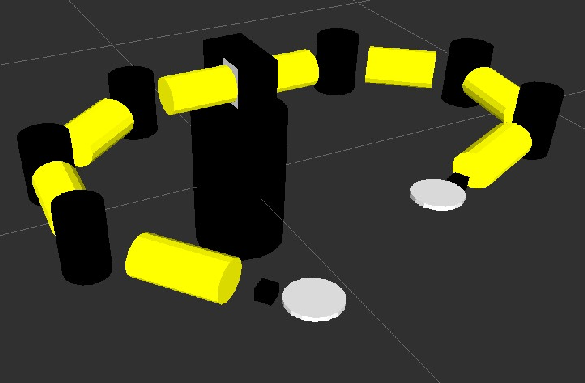
\includegraphics[width=1.0\columnwidth]{fig/robotModel-crop}
    \caption{
      The tailor made dual-arm robot model for the paddling simulation.
    }
     \label{fig:trajectory}
  \end{center}
\end{figure}


Please find more details in the code. 

\bibliographystyle{IEEEtran}
\bibliography{ref}
\end{document}

